\section{Initialization}

\subsection{Manual}
As suggested in the project statement, manual initialization
was implemented first to evaluate the fitting algorithm and
the automatic initialization separately.

The implementation is pretty straightforward. Using different
OpenCV routines, the mean shape can be dragged to its initial
position, and one it has been located, the fitting algorithm starts.

Nevertheless, this procedure presents a problem. The rotation of the
shape can't be changed, which causes that the initial estimation is not
as accurate as it could be.

\subsection{Automatic}

What really would make a difference in object detection is to make it automatic,
and not having to drag a shape, for each object to be detected, in each image.
Our first approach to make an automatic model was using histogram of oriented
gradients (HOG), combined with training a support vector machine (SVM), to
detect the shape of the 8 incisives altogether. But we stumbled upon an
obstacle. Whereas with other images (much more clear, less noise, with highly
detailed edges) this method is feasible, with our images it was not as good,
even after treating the image with techniques (such as denoising, white and
black hat...) The following images represent an example with a normal image, 
and one cropped section of incisives, from radiograph1.

\begin{figure}[h]
  \centering
  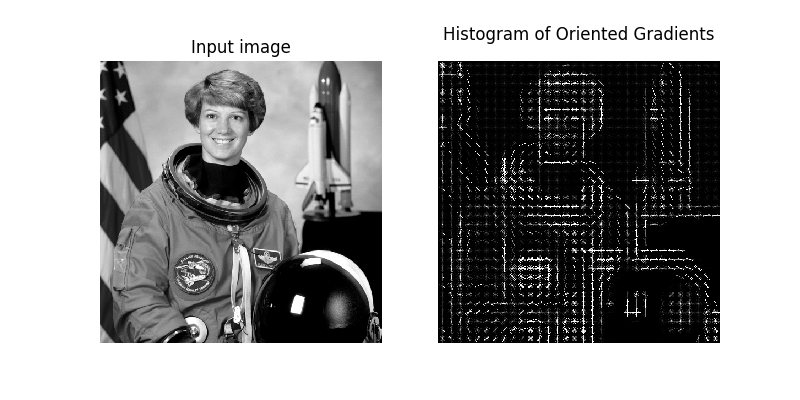
\includegraphics[height=6cm]{img/astro_hog}
  \caption{Normal image and its HOG}
\end{figure}

\begin{figure}[h]
  \centering
  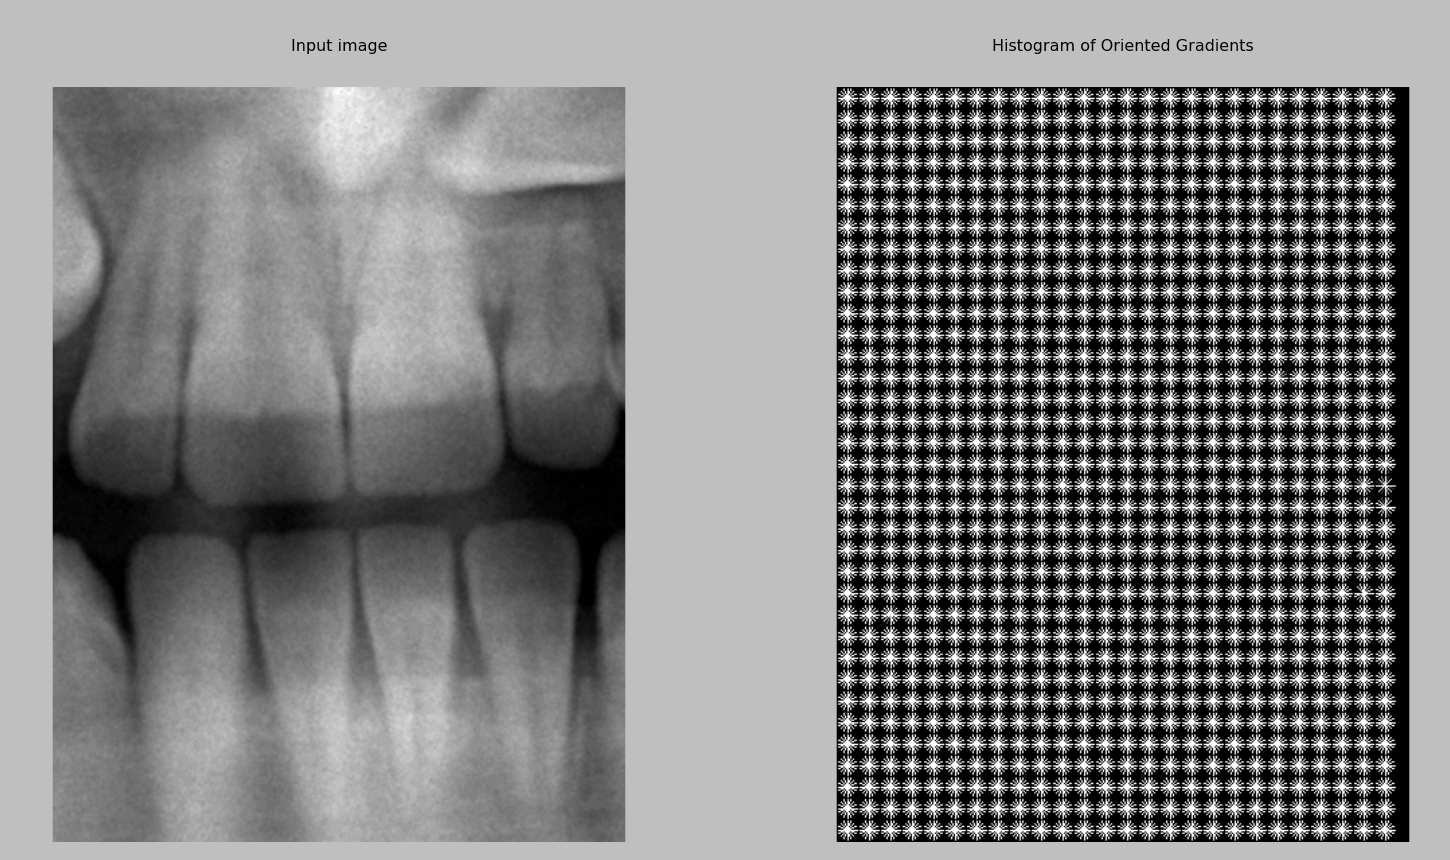
\includegraphics[height=5cm]{img/teeth_hog}
  \caption{Cropped teeth section}
\end{figure}

After that, we opted for using the Viola-Jones detection technique. With this
technique, some "basic" features are used to train a cascade classifier, which
consist of several "weak" classifiers, boosted by the appending of one afther
the other. 

In order to train the classifiers, sections such as the one shown in the figure
above were cropped from each of the 30 radiographs, for the positive data, and,
as for the negative data, 150 random images were gathered. Each image
(regardless positive or negative), was denoised and greyed before being used for
training. 

As for how the training was made, first, a \textit{out.vec} was created with the
tool \textit{opencv\_createsamples}, and the set of images, together with a list
of anotations for the positive samples. Once having the out.vec, the next step
is to use the tool \textit{opencv\_traincascade}, in order to create the
corresponding .xml file with the classifier. Due to the ammount of data not
being too large, we choose to make it a 3-stage classifier (more would have been
not efficient, due to the time to train it, and not improving too much, due to
having a low quantity of samples)

The results obtained are good enough, but not better. The gist of
the Viola-Jones technique is that it is quite fast, but it is not flawless, and
it found quite some false positives, as shown in the image below

\begin{figure}[h]
  \centering
  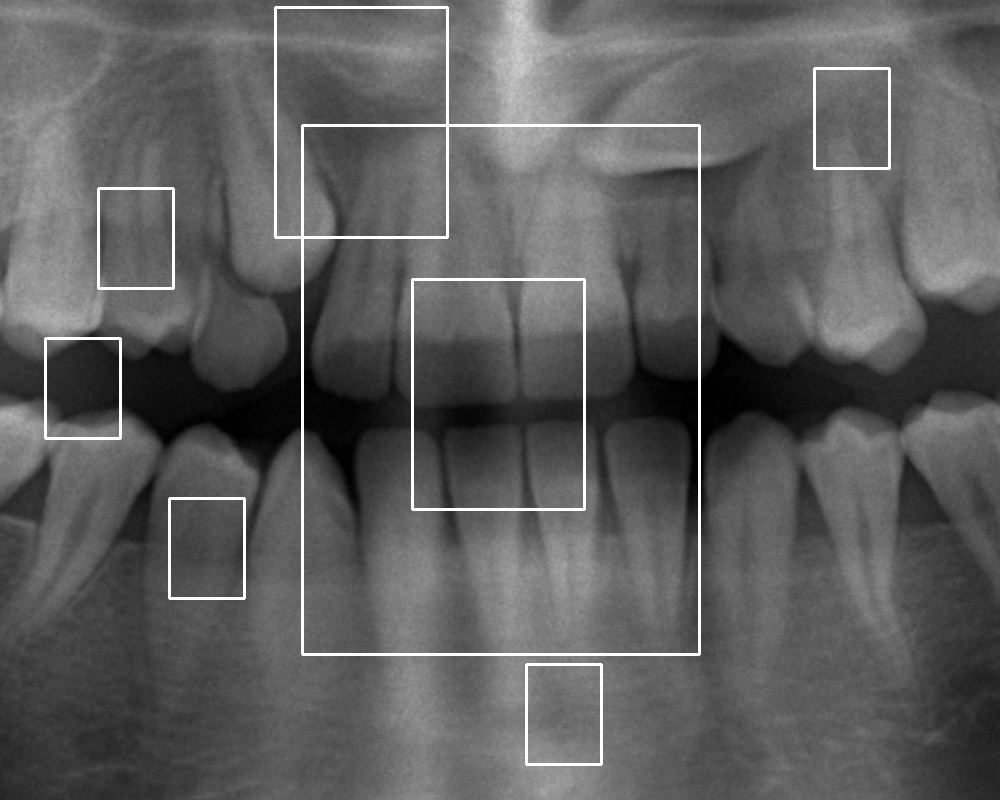
\includegraphics[height=6cm]{img/teeth_detection_1}
  \caption{Initial results of Viola-Janes detection}
\end{figure}

As can be seen, there is one very good match, and several bad matches. For this
matter, what we did in order to correct the results are two things, 
first, detection-wise, we tinkered with the detection parameters, changing the
scale at which the image would be resized for further detections, and the
minimum number of neighbours, which, if changed to a high value, it would result
in few detections, but of higher quality, which is what we are interested on.
Result-wise changes made to improve the detection were, first delete rectangles
that are inside of others, and then proceed to ignore those that are not
sufficiently large enough. With these two techniques, we have a result such as
this

\begin{figure}[h]
  \centering
  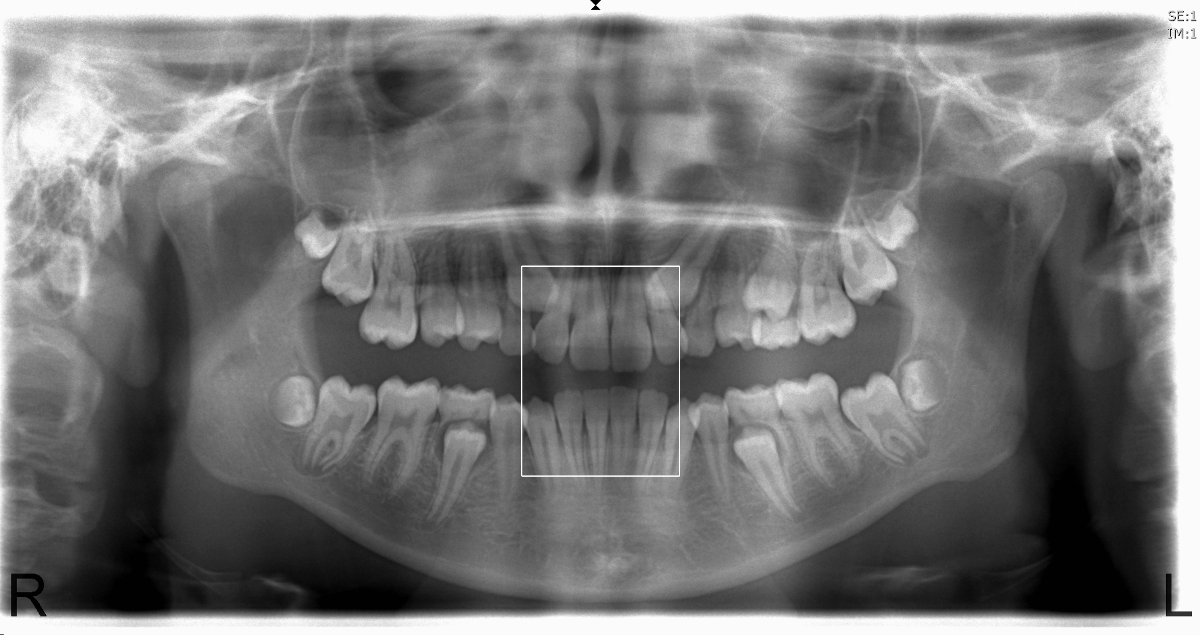
\includegraphics[height=6cm]{img/teeth_detection_2}
  \caption{Improved results}
\end{figure}

Once we have a proper automatic detector mechanism, all that remains is to place
the shape in its correct position. For this matter, a small choosing technique
was developed:
\begin{itemize}
  \item If the incisive is one of the upper four, the y position is located at
the first third of the rectangle. For the x centroid, the width is divided in 4,
and the centroid will be the center of one of them (corresponding to the
incisive)
  \item On the other hand, if the incisive is one of the lower four, the y
centroid is located slightly below the second third of the height. The x
position in this case is trickier. The lower incisives are usually smaller
(altogether) than the upper ones, so a different mechanism has to be made. For
this matter, instead of dividing the width by 4, it was dividived by 8, and the
first two, and the last two areas are not going to be selected. Meaning, the
incisives will be placed at one of the middle 4 areas, out of the division of 8
made.  
\end{itemize}
